%# -*- coding: utf-8-unix -*-
% !TEX program = xelatex
% !TEX root = ../thesis.tex
% !TEX encoding = UTF-8 Unicode
%%==================================================
%% chapter01.tex for SJTU Master Thesis
%%第二章
%%==================================================
\chapter{深度强化学习介绍}
深度强化学习是结合了深度学习算法和传统强化学习算法的结合体,下面分别介绍传统的强化学习算法理论基础知识,然后深入到深度强化学习进行几种典型的算法及应用。

\section{强化学习简介}
强化学习是一个由行为心理学引导出来的面向目标的机器学习领域。其研究的目标就是在和环境不断交互的过程中,经过一系列的决策过程达到累计奖励值最大化的过程。强化学习和监督学习的区别主要有一下两点:

不同于监督学习根据历史经验感知周围的环境,强化学习没有明确的标签信息,强化学习的学习机制是通过不断进行尝试和环境进行交互根据结果进一步优化决策信息实现的。可以说强化学习是一种具有标签延迟的监督学习。

监督学习的前提是数据独立同分布的,而强化学习本身没有这个约束,其模型的前提是数据基于高度序列化,智能体当前的动作会影响到下一时刻。

\subsection{强化学习基本概念}

强化学习的研究离不开以下几个组成成分:

\begin{enumerate}
	\item 智能体(Agent):智能体被定义为有智慧的决策体,也是我们最后需要学习的策略的承载体。在这里智能体就是强化学习算法最后学到的模型。
	\item 动作(Action,A): $ S=\{a_{0},a_{1},a_{2},\dots,a_{n}\} $行动是智能体采取动作的集合,智能体从动作列表集合里选取合适的动作,进行与周围环境的交互过程。在这里动作可以是离散的也可以是离散的。
	\item 环境(Environment):环境包含了智能体当前的状态和行为动作的输入。又会根据智能体选择动作的变化输出下一个状态和奖励反馈信息。通常环境蕴含了一定的物理模型规律或社会规则。
	\item 状态(State,S): $ S=\{s_{0},s_{1},s_{2},\dots,s_{n}\} $状态反应了智能体当前所处状态的特征,包括位置信息,角度信息,像素信息,等等。是通过环境反馈回来的。
	\item 奖励(Reward, R) :奖励是评估一个动作好坏的重要参数,对于现定的状态信息,当智能体选择动作和环境进行交互,环境转移到下一状态(新的状态受之前一系列动作状态转移过程的影响)的同时反馈回当前动作的奖励值,奖励值可以是即时的也可以是有时间延迟的。奖励分为正向收益和负向收益,在当前状态下,当鼓励某个动作的出现时,环境反馈出正向收益,反之当采取不合适的动作后,环境反馈出负向收益,也成为惩罚。${R_t}$ 代表当前时刻获取的即时奖励。
\end{enumerate}

强化学习的整体学习过程可以用图示 \ref{fig:1}表示。在每一个离散的时间点$t$,智能体将当前的环境状态${s_t}$和即时奖励${r_t}$作为输入,把下一时刻的行动概率作为输出。然后从允许的动作集合中选取合适的行动${{\rm{a}}_t}$,智能体下一时刻的动作反过来影响环境下一时刻的状态转移 $P({S_{t + 1}}|{S_t}) = P({S_1},...,{S_t})$,环境更新状态到${{\rm{s}}_{t + 1}}$,进而决定了和这个变化$\left( {{{\rm{s}}_t},{a_t},{s_{t + 1}}} \right)$相关的奖励${r_{t{\rm{ + }}1}}$。环境相当于黑盒模型,强化学习相当于智能体在学习逼近环境函数,从而得到最大的累积奖励。区别于其他监督学习和非监督学习,强化学习学习到的是一系列的先后发生的状态动作(state-action)对。

\begin{figure}[!htpb]
	\centering
	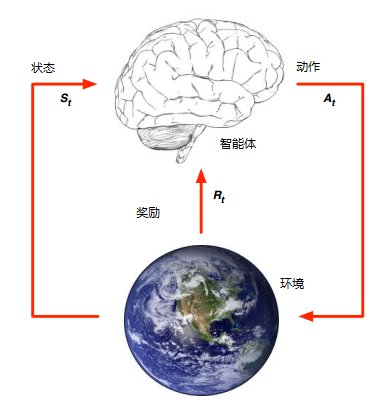
\includegraphics[width=10cm]{example/reinforcement_learning_pro.png}
	\bicaption[这里将出现在插图索引]
	{强化学习交互过程}
	{The history of Artificial Intelligence.}
	\label{fig:1}
\end{figure}
\subsection{有限马尔科夫决策过程}
绝大多数强化学习解决的问题都可以抽象为马尔科夫决策过程(Markov Decision Process, MDP)。在决策任务中,对于一个给定的策略,如果环境未来状态的概率分布只取决于当前环境本身,而与历史时刻信息无关,便具有马尔科夫性,其过程成为马尔科夫过程。马尔科夫决策过程由$(S,A,P,R,\gamma )$ 五个元素组成,其中,$S$ 为有限的状态集,$ A $为有限的动作集,$P$ 为状态转移概率,$ R $ 为回报函数,$\gamma$ 为折扣系数。马尔科夫决策过程描述的是这种无记忆的随机过程可以用下面的状态转移概率公式表达:
\begin{equation}
\label{eq:2}
{P_{ss'}} = P[{S_{t + 1}} = s'|{S_t} = s,{S_{t - 1}},...,{S_1}] = P[{S_{t + 1}} = s'|{S_t} = s]
\end{equation}

其中,$ P $代表状态转移矩阵,包含了所有状态之间转移的概率值:

\begin{equation}
P = \left[ {\begin{array}{*{20}{c}}
	{{P_{11}}}& \cdots &{{P_{1n}}}\\
	\vdots & \ddots & \vdots \\
	{{P_{n1}}}& \cdots &{{P_{nn}}}
	\end{array}} \right]
\end{equation}
$n$为状态的数量。
马尔科夫奖励过程引入了奖励函数$R$和折扣因子$\gamma$($\gamma  \in \left[ {0,1} \right)$),折扣系数代表从当前时刻对以后获得的所有奖励进行估计,距离当前时刻越远的即时奖励占的比重越小,$\gamma$越接近0,代表从当前状态往后看的步数越少,$\gamma$越接近1,代表从当前状态往后延申的比重越大,从某一时刻$0$往后直到当前幕结束所有累计奖励为:
\begin{equation}
\label{eq:resthm}
{{\rm{G}}_{\rm{t}}} = {R_{t + 1}} + \gamma {R_{t + 2}} + ... + \sum\limits_{k = 0}^\infty  {{\gamma ^k}{R_{t + k + 1}}} 
\end{equation}
期望回报表示为
\begin{equation}
\label{eq:e}
R_{ss'}^a = E[{r_{t{\rm{ + }}1}}{\rm{|}}{{\rm{S}}_t} = s,{S_{t + 1}} = s',{a_t} = a]
\end{equation}
这里引入两个求解MDP问题常用的概念:
\begin{enumerate}
	\item 策略(policy, $ \pi $):策略是智能体面临的决策,在这里强化学习建立在马尔可夫性的基础上,因此策略只依赖于当前状态,与前面时刻的动作状态无关,因此策略可以表示成一系列二元组:$\left \{ \left ( s_{1},a_{1} \right ),\left ( s_{2},a_{2}\right ),\left ( s_{3},a_{3}\right ),\dots,\left ( s_{n},a_{n}\right )\right \}$。策略可以认为在当前状态下采取某种行动的概率,其完整的表述了智能体的一系列决策过程。
\begin{equation}
\label{eq:3}
\pi (a|s) = P[{A_t} = a|{S_t} = s]
\end{equation}
	\item 值函数(value, v):正如前面提到的,强化学习建立决策过程是基于对当前状态的评估,称为值函数。值函数为智能体在折扣系数 $\gamma$的长期累积收益期望。
\end{enumerate}

值函数分为动作值函数$V$ 和状态动作值函数$Q$。在给定状态情况下,对于某一策略 $\pi$, 状态值函数表示直到结束当前过程所获得的累积收益:
\begin{equation}
\label{eq:4}
{v_\pi }(s) = {E_\pi }[{G_t}|{S_t} = s]
\end{equation}
动作值函数指智能体在当前状态下一直遵循策略$ \pi $,采取动作$a$,直到结束当前幕所获得的累积收益:
\begin{equation}
\label{eq:5}
{q_\pi }(s,a) = {E_\pi }[{G_t}|{S_t} = s,{A_t} = a]
\end{equation}
当某一策略的收益期望大于其他策略时,该策略成为最优策略,对应的值函数为最优值函数,最优状态值函数和最后动作-状态值函数表示为:

\begin{equation}
\label{eq:6}
{v_*}(s) = \mathop {\max }\limits_\pi  {v_\pi }(s)
\end{equation}

\begin{equation}
\label{eq:7}
{q_*}(s,a) = \mathop {\max }\limits_\pi  {q_\pi }(s,a)
\end{equation}
根据定理\ref{thm:马尔科夫定理}可知,最优策略总是存在并同时使得状态值函数和状态动作值函数取得最大值。
\begin{thm}[马尔科夫定理]
\label{thm:马尔科夫定理}
对于任意的马尔科夫决策过程:
\begin{enumerate}
	\item 存在一个最优的策略函数${\pi _{\rm{*}}}$使得最后的累积奖励大于其他策略$ \pi$。
	\item 该最优策略函数${\pi _{\rm{*}}}$使得状态值函数达到最大值:
	\begin{equation}
	\label{eq:optimal}
	{v_{{\pi _*}}}(s) = {v_*}(s)
	\end{equation}
	\item 该最优策略函数${\pi _{\rm{*}}}$同时使得状态-动作值函数达到最大值:
	\begin{equation}
	\label{eq:optimal}
	{q_{{\pi _*}}}(s,a) = {q_*}(s,a)
	\end{equation}
	
\end{enumerate}
\end{thm}

求解出最优值函数就解决了马尔科夫决策过程。通常对于状态转移函数已知的模型(model-based),可以通过贝尔曼期望方程求解最优函数:
\begin{equation}
\label{eq:bell1}
{v_\pi }(s) = {E_\pi }[{r_{t + 1}} + \gamma {r_{t + 2}} + {\gamma ^2}{r_{t + 3}} + ...|{S_t} = s] = {E_\pi }[\sum\limits_{k = 0}^\infty  {{\gamma ^k}{r_{t + k + 1}}|{S_t}}  = s]
\end{equation}

将第一步奖励提出来,整理得到:
\begin{equation}
\label{eq:bell3}
{v_\pi }(s) = {E_\pi }[{r_{t + 1}} + \gamma \sum\limits_{k = 0}^\infty  {{\gamma ^k}{r_{t + k + 2}}|{S_t}}  = s]
\end{equation}

其中期望奖励和可以由所有即时奖励累加得到:
\begin{equation}
\label{eq:bell4}
{E_\pi }[\gamma \sum\limits_{k = 0}^\infty  {{\gamma ^k}{r_{t + k + 2}}|{S_t}}  = s] = \sum\limits_a {\pi (s,a)\sum\limits_{s'} {p_{ss'}^a} } \gamma {E_\pi }[\sum\limits_{k = 0}^\infty  {{\gamma ^k}{r_{t + k{\rm{ + }}2}}{\rm{|}}{{\rm{S}}_{t + 1}} = s'} ]
\end{equation}

根据上述公式,方程整理为:
\begin{equation}
\label{eq:bell5}
{V_\pi }(s) = \sum\limits_a {\pi (s,a)\sum\limits_{s'} {p_{ss'}^a} } [R_{ss'}^a + \gamma {E_\pi }[\sum\limits_{k = 0}^\infty  {{\gamma ^k}{r_{t + k + 2}}|{S_{t + 1}}}  = s']]
\end{equation}
利用上一时刻的状态值函数替换\ref{eq:bell5}:
\begin{equation}
\label{eq:bell6}
{V_\pi }(s) = \sum\limits_a {\pi (s,a)\sum\limits_{s'} {p_{ss'}^a} } [R_{ss'}^a + \gamma {V_\pi }(s')]
\end{equation}
同理,动作状态值函数整理为:
\begin{equation}
\label{eq:bell7}
{Q_\pi }(s,a) = \sum\limits_{s'} {p_{ss'}^a} [R_{ss'}^a + \gamma {Q_\pi }(s')]
\end{equation}
相应的,状态值函数和状态动作值函数的最优方程为:
\begin{equation}
\label{eq:bell8}
{V_*}(s) = \mathop {\max }\limits_a \left( {{\rm{R}}_s^a + \gamma \sum\limits_{s' \in S} {P_{ss'}^a{V_*}(s')} } \right)
\end{equation}
\begin{equation}
\label{eq:bell9}
{Q_*}(s,a) = {\rm{R}}_s^a + \gamma \sum\limits_{s' \in S} {P_{ss'}^a\mathop {\max }\limits_{a'} {Q_*}(s',a')}
\end{equation}
\subsection{基于价值函数的算法}
以上介绍的方程最优解法都是有模型学习,也就是状态转移函数是已知的,对于免模型式的强化学习可以用基于价值函数的算法求解。典型的基于价值函数求解的算法包括蒙特卡洛(Monte Carlo,MC)\cite{singh1996reinforcement}和时序差分(Temporal-Difference,TD)\cite{tesauro1995temporal}。两种算法都是基于已有的历史数据对价值函数进行更新。

蒙特卡洛是回合制更新,需要等到一个回合结束后对所有的动作进行值函数的更新如图\ref{fig:5}:
\begin{figure}[htpb]
	\centering
	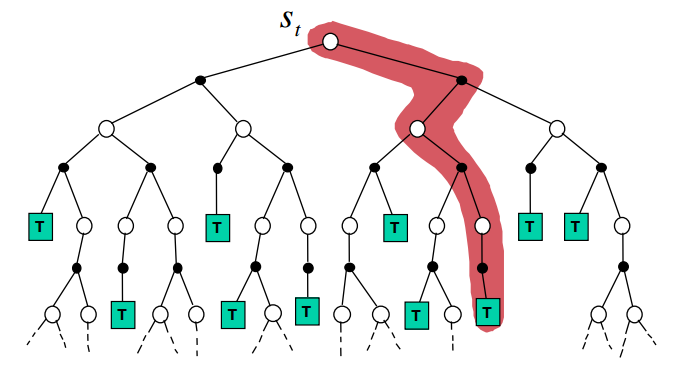
\includegraphics[width=15cm]{example/MC.png}
	\bicaption[这里将出现在插图索引]
	{蒙特卡洛值函数更新方式示意图}
	{The history of Artificial Intelligence.}
	\label{fig:5}
\end{figure}
MC的更新方式如下:
\begin{equation}
\label{eq:mc}
V({S_t}) \leftarrow V({S_t}) + \alpha [{G_t} - V({S_t})]
\end{equation}
在这里,$\alpha$ 是学习率,也就是更新步长。蒙特卡洛算法通过大量的与环境进行交互获取历史经验信息,通过这些信息近似的估计状态值函数。对于下一次迭代,智能体会根据上一轮的状态值函数选择新的动作,直到收敛。一个典型的蒙特卡洛强化学习算法如\ref{algo:MC}:

\begin{algorithm}
	% \begin{algorithm}[H] % 强制定位
	\caption{蒙特卡洛强化学习算法}
	\label{algo:MC}
	\begin{algorithmic}[1] %每行显示行号
		\State 初始化$Q(s,a) = 0,count(s,a) = 0,\pi (s,a) = \frac{1}{{|A(s)|}}$
		\For {回合$episode = 1 \to N$}
		\State 在环境中执行策略$\pi$,同时记录轨迹$\left\langle {({s_1},{a_1},{r_1}),({s_2},{a_2},{r_2}),...,({s_T},{a_T},{r_T})} \right\rangle  $
		
		\For{$t = 0 \to T-1$}
		\State $R = \frac{1}{{T - t}}\sum\nolimits_{i = t + 1}^T {{r_i}} $
		\State $Q({s_t},{a_t}) = \frac{{Q({s_{\rm{t}}},{a_t}) \times count({s_t},{a_t}) + R}}{{count({s_t},{a_t}) + 1}} $
		\State $count({s_t},{a_t}) = count({s_t},{a_t}) + 1$
		\EndFor
		\State 对于所有已经历过的状态s:
		      
		      策略$\pi (s,a)$更新为$\varepsilon $贪心地选择$\arg {\max _{a'}}Q(s,a')$
		\EndFor
	\end{algorithmic}
\end{algorithm}
在每一次迭代过程中,先让智能体完整的进行一次回合训练,并记录相应的轨迹$\left\langle {({s_1},{a_1},{r_1}),({s_2},{a_2},{r_2}),...,({s_T},{a_T},{r_T})} \right\rangle  $,然后对每一个状态动作对$({s_t},{a_t}) $计算平均累计收益:
\begin{equation}
\label{eq:reward}
R = \frac{1}{{T - t}}\sum\nolimits_{i = t + 1}^T {{r_i}} 
\end{equation}
再用所有累计收益除以每个状态访问的次数就是当前状态动作对的平均收益,这个平均收益就是估计的值函数:
\begin{equation}
\label{eq:reward2}
Q({s_t},{a_t}) = \frac{{Q({s_{\rm{t}}},{a_t}) \times count({s_t},{a_t}) + R}}{{count({s_t},{a_t}) + 1}} 
\end{equation}
TD算法是单步更新制,只需要等下一时刻状态的到来即可利用下一时刻的奖励$ {R_{t + 1}}$和值函数$V({S_{t + 1}}) $进行值函数的更新操作。\ref{fig:6}为TD算法更新方式。
\begin{figure}[htpb]
	\centering
	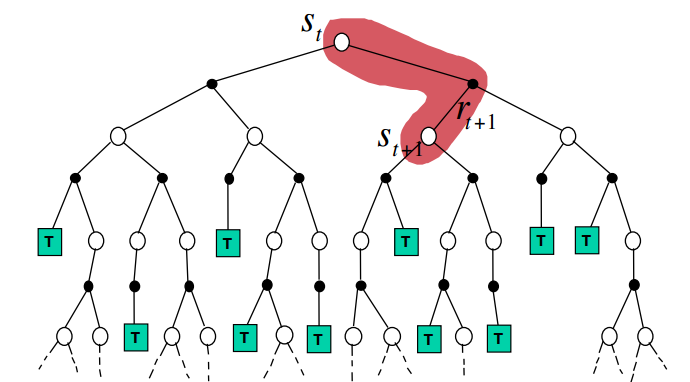
\includegraphics[width=15cm]{example/TD.png}
	\bicaption[这里将出现在插图索引]
	{单步差分值函数更新方式示意图}
	{The history of Artificial Intelligence.}
	\label{fig:6}
\end{figure}
TD的更新方式如下:
\begin{equation}
\label{eq:td}
V({S_t}) \leftarrow V({S_t}) + \alpha [{R_{t + 1}} + \gamma V({S_{t + 1}}) - V({S_t})]
\end{equation}
典型的基于TD算法的基于值函数更新的算法有Q-learning算法和Sarsa算法。其算法逻辑分别为\ref{algo:Q}和\ref{algo:sarsa}。

\begin{algorithm}
	% \begin{algorithm}[H] % 强制定位
	\caption{Q-learning算法}
	\label{algo:Q}
	\begin{algorithmic}[1] %每行显示行号
		\State 初始化$Q(s,a) = 0,\pi (s,a) = \frac{1}{{|A(s)|}},s = {s_0}$
		\For {回合$episode = 1 \to N$}
		\State 输入当前环境状态
		  \For {当前回合没有结束}
		  \State 
		根据当前最新的值函数$Q$和状态$ s $,使用$\epsilon - greddy$策略得到动作$ a $
		  \State 执行动作$ a$,得到即时奖励$r$和新的状态$ s'$
		  \State 更新$ Q $值:$ Q(s,a) \leftarrow Q(s,a) + \alpha [r + \gamma \mathop {\max }\limits_{a'} Q(s',a') - Q(s,a)]$
		  \State 更新状态:$s \leftarrow s'$
		  \EndFor
		\EndFor
	\end{algorithmic}
\end{algorithm}

\begin{algorithm}
	% \begin{algorithm}[H] % 强制定位
	\caption{Sarsa算法}
	\label{algo:sarsa}
	\begin{algorithmic}[1] %每行显示行号
		\State 初始化$Q(s,a)$ = 0
		\Repeat 
		\State 输入当前环境状态
		\State 根据当前最新的值函数$Q$和状态$ s $,使用$\epsilon - greddy$策略得到动作$ a $
		\For {对于当前回合每一步动作}
		\State 执行动作$ a$,得到即时奖励$r$和新的状态$ s'$
		\State 根据当前最新的状态$ s' $,使用$\epsilon - greddy$策略得到新的动作$ a' $
		\State 更新$ Q $值:$ Q(s,a) \leftarrow Q(s,a) + \alpha [r + \gamma Q(s',a') - Q(s,a)]$
		\State 更新状态:$s \leftarrow s'$,:$a \leftarrow a'$
		\EndFor
		\Until{进行完所有的回合数}
	\end{algorithmic}
\end{algorithm}
对于以上两种算法,可以看出区别在于对动作选择的方式不一样,Sarsa是在线学习方式,根据策略选择出的动作即是最后执行的动作,而Q-learning算法引入了贪心策略,选择Q值最大的那个动作作为最后执行的动作。

如图\ref{fig:4},TD算法是单步更新,因此更新速率较快,但是由于其更新的目标基于下一步的估计值,更新的方向只取决于下一步的值,估计会带来偏差,因此更新后的价值函数具有高偏差低方差的特性。MC算法是基于回合更新的,其更新的方法取决于本回合所有实际得到的奖励值,因此更新的速度更慢,具有较高的波动,因此MC具有低偏差,高方差的特性。
\begin{figure}[htpb]
	\centering
	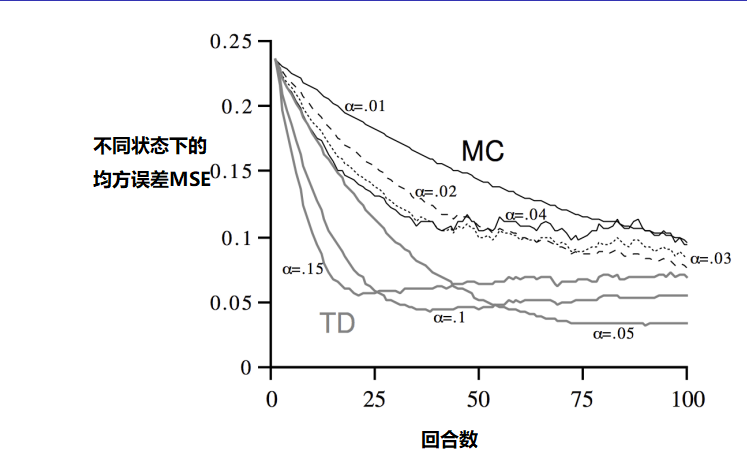
\includegraphics[width=15cm]{example/MC_and_TD.png}
	\bicaption[这里将出现在插图索引]
	{MC和TD误差随迭代次数变化曲线}
	{The history of Artificial Intelligence.}
	\label{fig:4}
\end{figure}
\subsection{基于策略梯度的算法}
上述介绍的价值函数的算法是先得到每一状态的得分,然后智能体选取得分最高的动作进行下一步策略的选择,还有一种方法是不依靠于值函数,输入是当前的状态,输出是下一步的动作或动作的概率值,这种学习方式称之为基于策略梯度的学习算法。和值函数更新的算法进行对比,值函数更新算法是确定性策略算法,一般结合$\varepsilon - greedy$ 算法进行探索避免陷入局部最优,在很多应用场景,动作的选择可能不是唯一的,某几种动作都是合理的,这时候输出所有动作的概率值就会变得更加合理。同时会防止方程陷入局部最优解。对于单步的MDP过程来说,从当前状态$S$开始选择一个动作$a$,得到当前状态的即时奖励$ r = R({\rm{s}},a) $,因为最后的目的是最大化奖励,因此优化的目标函数是$r$本身,即:
\begin{equation}
J(\theta ){\rm{ = }}{{\rm{E}}_\pi }[r] = \sum\limits_{s \in {\rm{S}}} {d(s)\sum\limits_{a \in A} {\pi (a|s;\theta )} } R(s,a)
\end{equation}

其中${\pi (a|s;\theta )}$是参数为$\theta$的策略网络。对目标函数求导:
\begin{equation}
\begin{split}
{\nabla _\theta }J(\theta ) =& \sum\limits_{s \in S} {d(s)\sum\limits_{a \in {\rm{A}}} {\pi (a|s;\theta )} } \frac{{{\nabla _\theta }\pi (a|s;\theta )}}{{\pi (a|s;\theta )}}R(s,a) \\
=& \sum\limits_{s \in S} {d(s)\sum\limits_{a \in {\rm{A}}} {\pi (a|s;\theta )} } {\nabla _\theta }\log \pi (a|s;\theta )R(s,a) \\
=& {E_\pi }[{\nabla _\theta }\log \pi (a|s;\theta )R(s,a)]
\end{split}
\end{equation}
可以看出最后目标函数的梯度是由两部分组成,一部分是策略函数对数梯度和即时奖励两部分乘积的期望值。以上是单步MDP过程的求解过程,对于多步MDP:
\begin{equation}
{\nabla _\theta }J(\theta ) = {E_\pi }[{\nabla _\theta }\log \pi (a|s;\theta ){Q_\pi }(s,a)]
\end{equation}
同样,基于策略梯度算法的强化学习也可以采用蒙特卡洛方法进行求解。也称为REINFORCE算法\cite{williams1992simple}。其算法如下:
\begin{algorithm}
	% \begin{algorithm}[H] % 强制定位
	\caption{REINFORCE算法}
	\label{algo:REINFORCE}
	\begin{algorithmic}[1] %每行显示行号
		\State 初始化网络参数$ \theta$ 
		\For {对于每一回合根据当前策略$\pi$得到走过每一步的$\{ {s_0},{a_0},{r_1},...,{s_{T - 1}},{A_{T - 1}},{R_T}\} $}
		\For{$t = 0 \to T-1$}
		\State 更新参数:$ \theta  \leftarrow \theta  + \alpha {\nabla _\theta }{G_t}\log \pi ({A_t}|{S_t};\theta )$
		\EndFor
		\EndFor
	\end{algorithmic}
\end{algorithm}
以上是传统强化学习的三种求解算法,对于复杂场景,对于外界环境的感知和特征提取能力显得尤为重要,对于函数拟合部分也越发变得困难,由此衍生了将强化学习模型和深度学习模型结合的深度强化学习模型。
\section{深度强化学习常见算法模型}
正如上文所述,对于免模型学习,强化学习最优方程的求解可以有基于价值网络和基于策略梯度以及结合价值网络和策略梯度同时进行求解的算法。结合深度学习模型也相应的延生出了两种基本的深度强化学习模型。下面分别介绍这两种种算法。
\subsection{Deep Q-learning算法介绍}
作为离线学习的值函数更新方法,Q-learning学习方法被广泛用于不同强化学习场景。通常简单的Q-learnig中状态动作价值函数$Q(s,a)$通常以表格的形式给出来。如图\ref{fig:8},行代表不同的状态,列代表在对应状态下可选择的动作。
\begin{figure}[htpb]
	\centering
	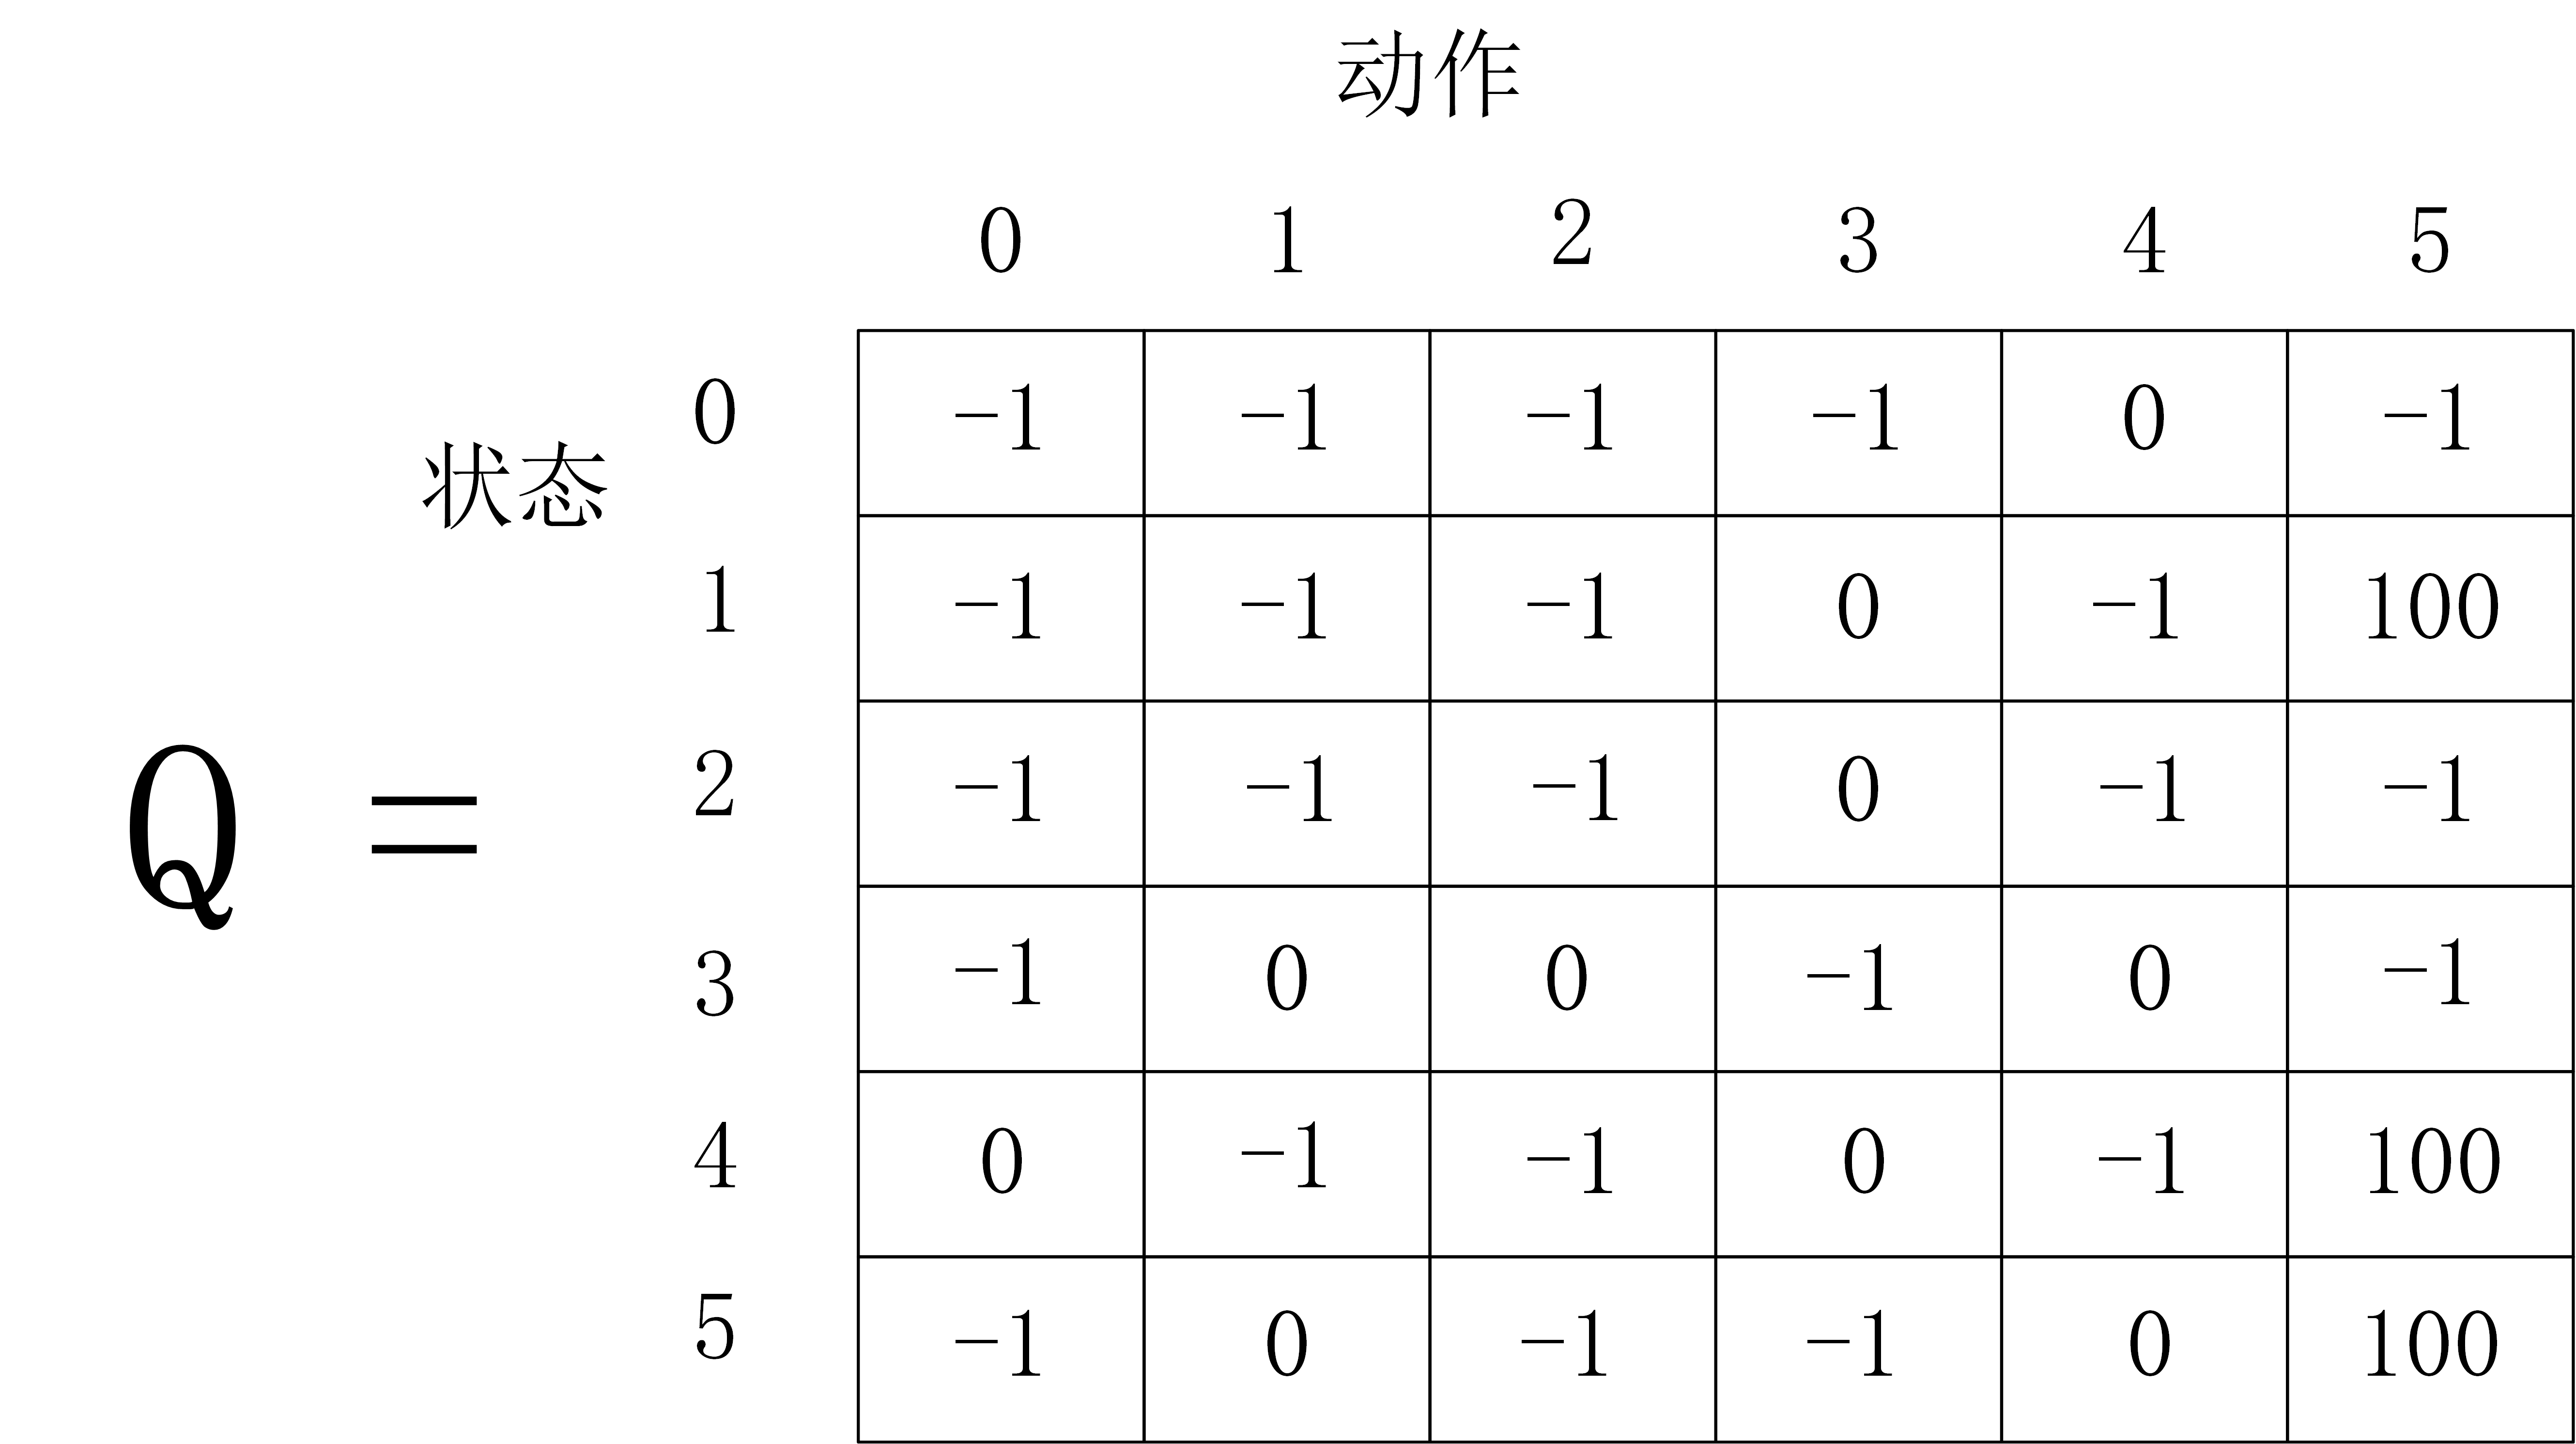
\includegraphics[width=15cm]{example/Q_table.jpg}
	\bicaption[这里将出现在插图索引]
	{Q值表示意图}
	{The history of Artificial Intelligence.}
	\label{fig:8}
\end{figure}
从上一节介绍可知,随着环境复杂度和动作可选范围增加,状态空间和动作空间的笛卡尔积尺寸变大,需要优化的状态动作值函数计算复杂度呈指数级数增长。对于高维的环境特征信息,如在图像视频领域,Q-learning算法不再适用,将深度学习网络应用在Q-learning框架下作为价值函数的逼近器代替传统的Q表想法应运而生,这种算法就是深度Q价值网络(Deep Q-learning,DQN)。DQN算法可以直接从原始输入状态中学习环境特征,返回值函数。DQN认为真实的Q值函数近似等于深度学习网络输出的值:
\begin{equation}
	{\rm{Q}}(s,a) \approx Q(s,a;\theta )
\end{equation}
其中,$\theta $为深度学习网络参数。DQN网络参数通过损失函数的最小化学到:
\begin{equation}
\label{eq:DQN}
L(\theta ) = \frac{1}{2}{(y - Q(s,a;\theta ))^2}
\end{equation}
这里面$y$为神经网络拟合的标签信息,对应于Q-learning中对目标的估计:
\begin{equation}
y = r + \gamma {\max _{a'}}Q({\rm{s'}},a';\theta )
\end{equation}
带入\ref{eq:DQN}:
\begin{equation}
\label{eq:DQN2}
	{\nabla _\theta }L(\theta ) = (r + \gamma \mathop {\max }\limits_{a'} Q(s',a';\theta ) - Q(s,a;\theta )){\nabla _\theta }Q(s,a;\theta )
\end{equation}
DQN做的另一个改进是数据的存取过程,DQN引入了经验回放技术,提高了样本的利用率,一定程度上减少了计算机的负担。每一个时刻智能体与环境交互产生的数据$ \left\langle {{s_t},{a_t},{r_{t + 1,}}{{\rm{s}}_{t + 1}}} \right\rangle $ 都存储在经验池中,在深度学习网络训练过程中每次参数的更新都会随机从经验出中采样出一个小批量样本进行学习。之后智能体再次采用随机-贪心算法进行动作的选择,DQN的算法如\ref{algo:DQN}所示。

\begin{algorithm}
	% \begin{algorithm}[H] % 强制定位
	\caption{DQN算法}
	\label{algo:DQN}
	\begin{algorithmic}[1] %每行显示行号
		\State 初始化Q网络参数更新的频率$C$,Q网络的参数$\theta$,最终输出目标网络参数$\theta ' = \theta $
		\For {回合数从1到$ M $}
		\State 初始化状态$ {s_1}$
		\For {动作步数从1到时刻$ T$}
		\State 根据当前最新的状态$ {s_t}$,使用$\epsilon - greddy$策略得到新的动作$a_t $
		\State 执行$a_t $,获取最新的奖励$ r_t+1 $,到达新的状态$ {s_t+1}$
		\State 将收集到的状态动作和奖励数据$ \left\langle {{s_t},{a_t},{r_{t + 1,}}{{\rm{s}}_{t + 1}}} \right\rangle $存储在经验池中
		\State 从经验池中随机采样mini-batch大小的数据$ \left\langle {{s_j},{a_j},{r_{j + 1,}}{{\rm{s}}_{j + 1}}} \right\rangle $,对于每一条数据计算估计Q值$y$:$ {y_j} = \left\{ {\begin{array}{*{20}{c}}
			{{{\rm{r}}_j}{\rm{,end}}}\\
			{{r_j} + \gamma \mathop {\max }\limits_{a'} \hat Q({s_{j + 1}},a';\theta '),not}
			\end{array}} \right.$
		\State 以公式\ref{eq:DQN2}为损失函数,对网络参数进行梯度下降更新。
		\State 以C为更新频率进行网络权重的更新$\theta ' = \theta $。
		\EndFor
		\EndFor
	\end{algorithmic}
\end{algorithm}
\subsection{Actor-Critic策略梯度算法}
蒙特卡洛策略梯度算法通过每一回合的完整更新,计算出来总的奖励价值往往相对准确,但是方差较大。如果通过值函数引导策略的更新,策略又反过来影响值函数的更新,这样两者相结合相互影响,学习的效果相对较好,这就是演员-评论家模型(Actor-Critic,AC)。

在这里引入优势函数(advantage function)的概念,优势函数代表当智能体在$t$时刻采取$a_t$ 动作后达到的状态要比当前状态$s_t$的总体平均价值好多少,公式表示为:

\begin{equation}
{A_\pi }(s,a) = {Q_\pi }(s,a) - {V_\pi }(s)
\end{equation}
Actor-Critic模型的损失函数可以引入优势函数:
\begin{equation}
\label{eq:ac}
J(\theta ) = {E_\pi }[\log \pi (a|s;\theta ){A_\pi }(s,a)]
\end{equation}
这里需要知道两个参数,${V_\pi } $和$ {Q_\pi } $,利用TD更新优势函数,把动作状态值函数转化为状态值函数,这样优势函数的TD误差变为:
\begin{equation}
\label{eq:error}
{\delta _\pi } = r + \gamma {V_\pi }(s') - {V_\pi }(s)
\end{equation}
利用\ref{eq:error}公式更新策略网络梯度\ref{eq:ac}:
\begin{equation}
\label{eq:error}
{\nabla _\theta }J(\theta ) = {\nabla _\theta }\log \pi (A|s;\theta )(r + \gamma V(s';{\theta _v}) - V(s;{\theta _v})) = \delta {\nabla _\theta }\log \pi (A|s;\theta )
\end{equation}

\begin{figure}[htpb]
	\centering
	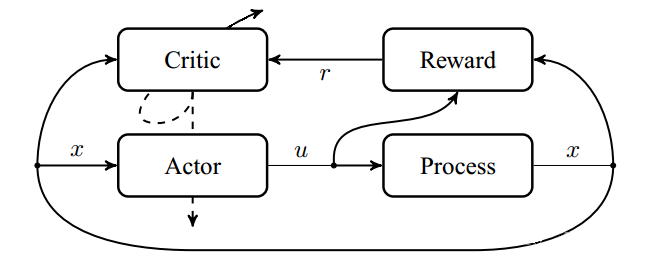
\includegraphics[width=15cm]{example/ac.png}
	\bicaption[这里将出现在插图索引]
	{Actor-Critic策略梯度算法更新过程}
	{The history of Artificial Intelligence.}
	\label{fig:ac}
\end{figure}
如图\ref{fig:ac}所示,Actor-Critic模型由两个部分组成:Actor基于动作概率选择下一步的动作,Critic根据当前的状态和Actor选择的动作获得的数据进行采样,逼近值函数进行打分,在下一次迭代中,Actor又会根据Critic打分值沿着最大化收益的方向改变动作概率输出。相对于传统的值函数更新,AC模型引入了策略梯度进行智能体策略的监督,使得训练更加稳定,同时AC模型利用TD方法进行优化函数的更新,弥补了蒙特卡洛策略梯度回合制更新方差大训练时间长的不足。AC模型的算法过程如下:

\begin{algorithm}
	% \begin{algorithm}[H] % 强制定位
	\caption{Actor-Critic策略梯度算法}
	\label{algo:DQN}
	\begin{algorithmic}[1] %每行显示行号
		\State 初始化策略网络参数和价值网络参数
		\For {回合数从1到$ M $}
		\State 初始化状态$ {s}$
		\For {动作步数从1到时刻$ T$}
		\State 根据当前最新的状态$ {s}$作为策略网络的输入,策略网络的输出为动作概率分布,依概率选择一个动作$ a_t $
		\State 执行$a_t $,获取最新的奖励$ r_t+1 $,到达新的状态$ {s'}$
		\State 计算TD误差${\delta _\pi } = r + \gamma {V_\pi }(s') - {V_\pi }(s)$
		\State 更新状态价值网络:${\theta _v} \leftarrow {\theta _v} + \beta \delta {\nabla _{{\theta _v}}}V(s;{\theta _v})$,其中,$\beta$ 为学习率
		\State 更新策略网络:$\theta  \leftarrow \theta  + \alpha \delta {\nabla _\theta }\log \pi (A|s;\theta )$,其中,$\alpha$ 为学习率
		\State 更新状态:$ s \leftarrow s'$
		\EndFor
		\EndFor
	\end{algorithmic}
\end{algorithm}

\section{本章小结}
本章第一部分首先介绍了强化学习了理论基础知识,与监督学习和无监督学习进行了对比,然后引入了强化学习基本的组成,强化学习中智能体和环境的交互过程,对于马尔可夫过程的求解,有两种方式,一种是回合更新制的蒙特卡洛算法,一种是单步更新的差分算法。对比两种方法的原理后发现各有利弊:蒙特卡洛算法偏差小而方差大,差分算法偏差大而方差小。根据强化学习动作选择的依据又可以分为基于值函数的强化学习和基于策略梯度的强化学习。基于值函数更新的强化学习算法主要基于状态值函数或者状态动作值函数对当前时刻状态进行评分,然后确定下一步动作的选择。常用的值函数更新的强化学习包括在线学习的Sarsa算法和离线学习的Q-learning算法。基于策略梯度更新算法,主要根据当前状态输出各个可能动作的概率值,对于连续型决策任务比较有效,传统的基于策略梯度更新的强化学习中主要为REINFORCE算法,对于单步更新和多布更新的损失函数文中都有相应介绍。本章的第二部分在第一部分相应理论知识的基础上引入了深度强化学习的概念,深度强化学习结合了深度学习的感知和特征提取能力和强化学习的决策能力,这一部分主要介绍了两种深度强化学习的算法:DQN算法和Actor-Critic算法。DQN在Q-learning算法的基础上,把传统的Q表替换为深度学习网络,深度学习作为函数的逼近器具有更强的泛化能力和函数拟合的能力同时引入了经验池的使用消除了数据时间上的关联性,同时增加了数据了利用效率。Actor-Critic策略梯度算法结合了值函数更新算法可以准确估计当前状态评分和策略梯度下降法能够有效使用TD算法进行连续快速更新的优势,Actor-Critic主要由状态值网络和策略网络构成,通过估计状态值函数给当前状态下的各个动作进行打分,策略网络根据状态值重新评估各个动作概率值进行更新。

本章在介绍强化学习基础知识后详细介绍了5种常用的算法并剖析他们各自的利弊,为后续章节奠定了理论基础。
